%%%%%% DON'T MODIFY STARTING HERE
\newpage
\section*{4.ROS Integration}

\paragraph{4A.} Install ROS kinetic \href{http://wiki.ros.org/Installation}{here}. Be sure to select the ``kinetic" tab after clicking on the platform option.
Make sure to activate the \texttt{52-O} conda environment we created earlier.
Attach screenshot of successful installation.

\paragraph{4B.} Install relevant ROS packages. Make sure to activate the \texttt{52-O} conda environment we created earlier.
Attach screenshot of successful installation.
\begin{itemize}
    \item \texttt{ros-kinetic-serial}
    \item \texttt{ros-kinetic-ros-control }
    \item \texttt{ros-kinetic-ros-controllers }
    \item \texttt{ros-kinetic-moveit }
    \item \texttt{ros-kinetic-gazebo-ros-pkgs }
    \item \texttt{ros-kinetic-gazebo-ros-control}
\end{itemize}

\paragraph{4C.} Replicate \textbf{1E} and \textbf{1F} using ROS. Reference the \href{https://document.wlkata.com/?doc=/wlkata-mirobot-resources-for-education/ros/ }{wlkata documentation} and \href {https://github.com/wlkata/RosForMirobot-master}{github repo}. Submit photo result in the space provided.
%%%%%% DON'T MODIFY UNTIL HERE
 
\newpage
\paragraph{Answers.}
Please do not exceed the height provided for each answer image.
%%%%%% YOU ANSWER STARTS HERE

% NOTE: MAKE SURE YOU DON'T CHANGE THE HEIGHT OF IMAGES
% NOTE: MAKE SURE TO REMOVE THE 'draft' OPTION FOR includegraphics BELOW. OTHERWISE, YOU WILL NOT SEE YOUR IMAGES.

\paragraph{4A. Install ROS kinetic.}

*Note on 4A and B: ROS is already installed on the Linux system in scili for all users so no additional steps are needed.

\begin{center}
    \includegraphics[draft,height=2.5in]{YOUR\_ANSWER.png}
\end{center}

\paragraph{4B. Install ROS Packages.}

* As noted in the previous question. ROS is already fully loaded for all users on the machine.

\begin{center}
    \includegraphics[draft,height=2.5in]{YOUR\_ANSWER.png}
\end{center}

\newpage
\paragraph{4C. Inverse Kinematics}
\begin{center}
    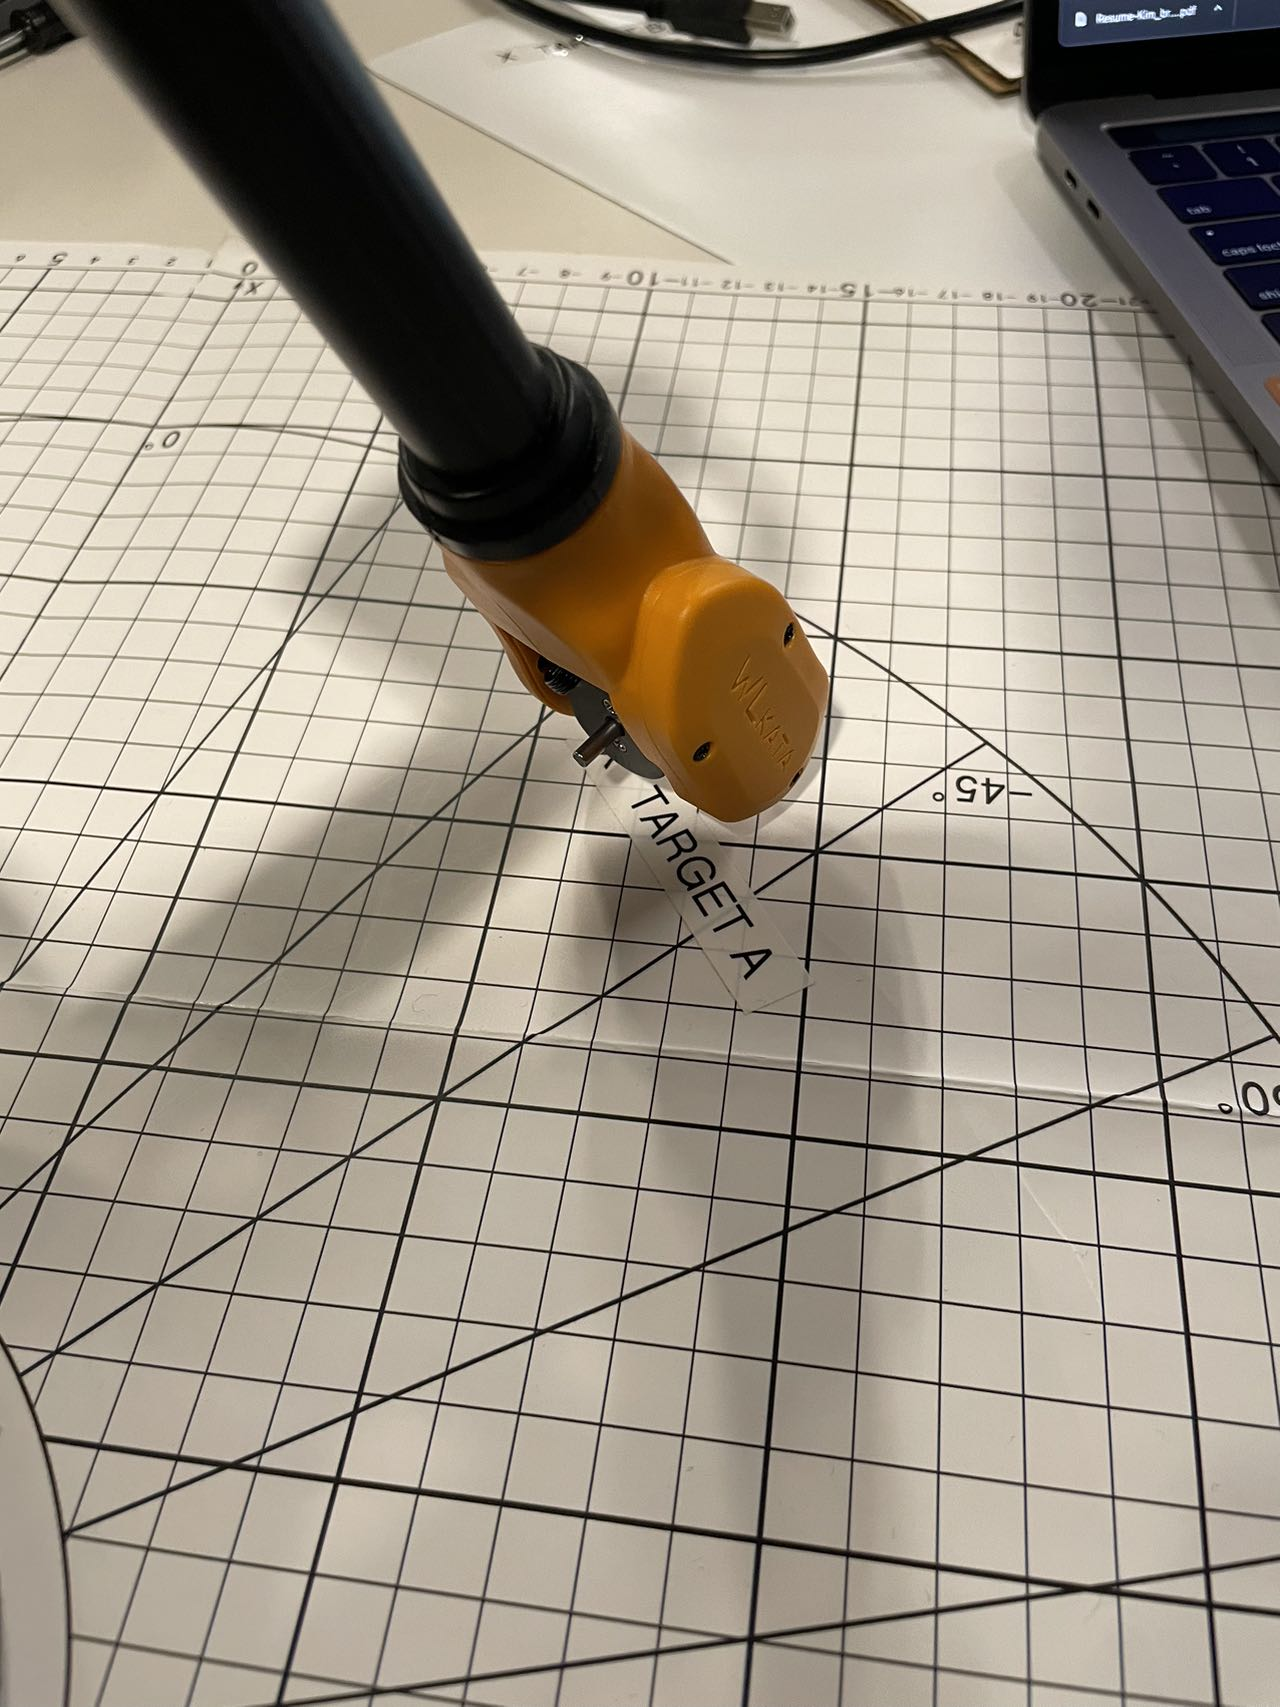
\includegraphics[height=2.5in]{image/4c_a.jpg}
\end{center}

\paragraph{4C. Forward Kinematics}
\begin{center}
    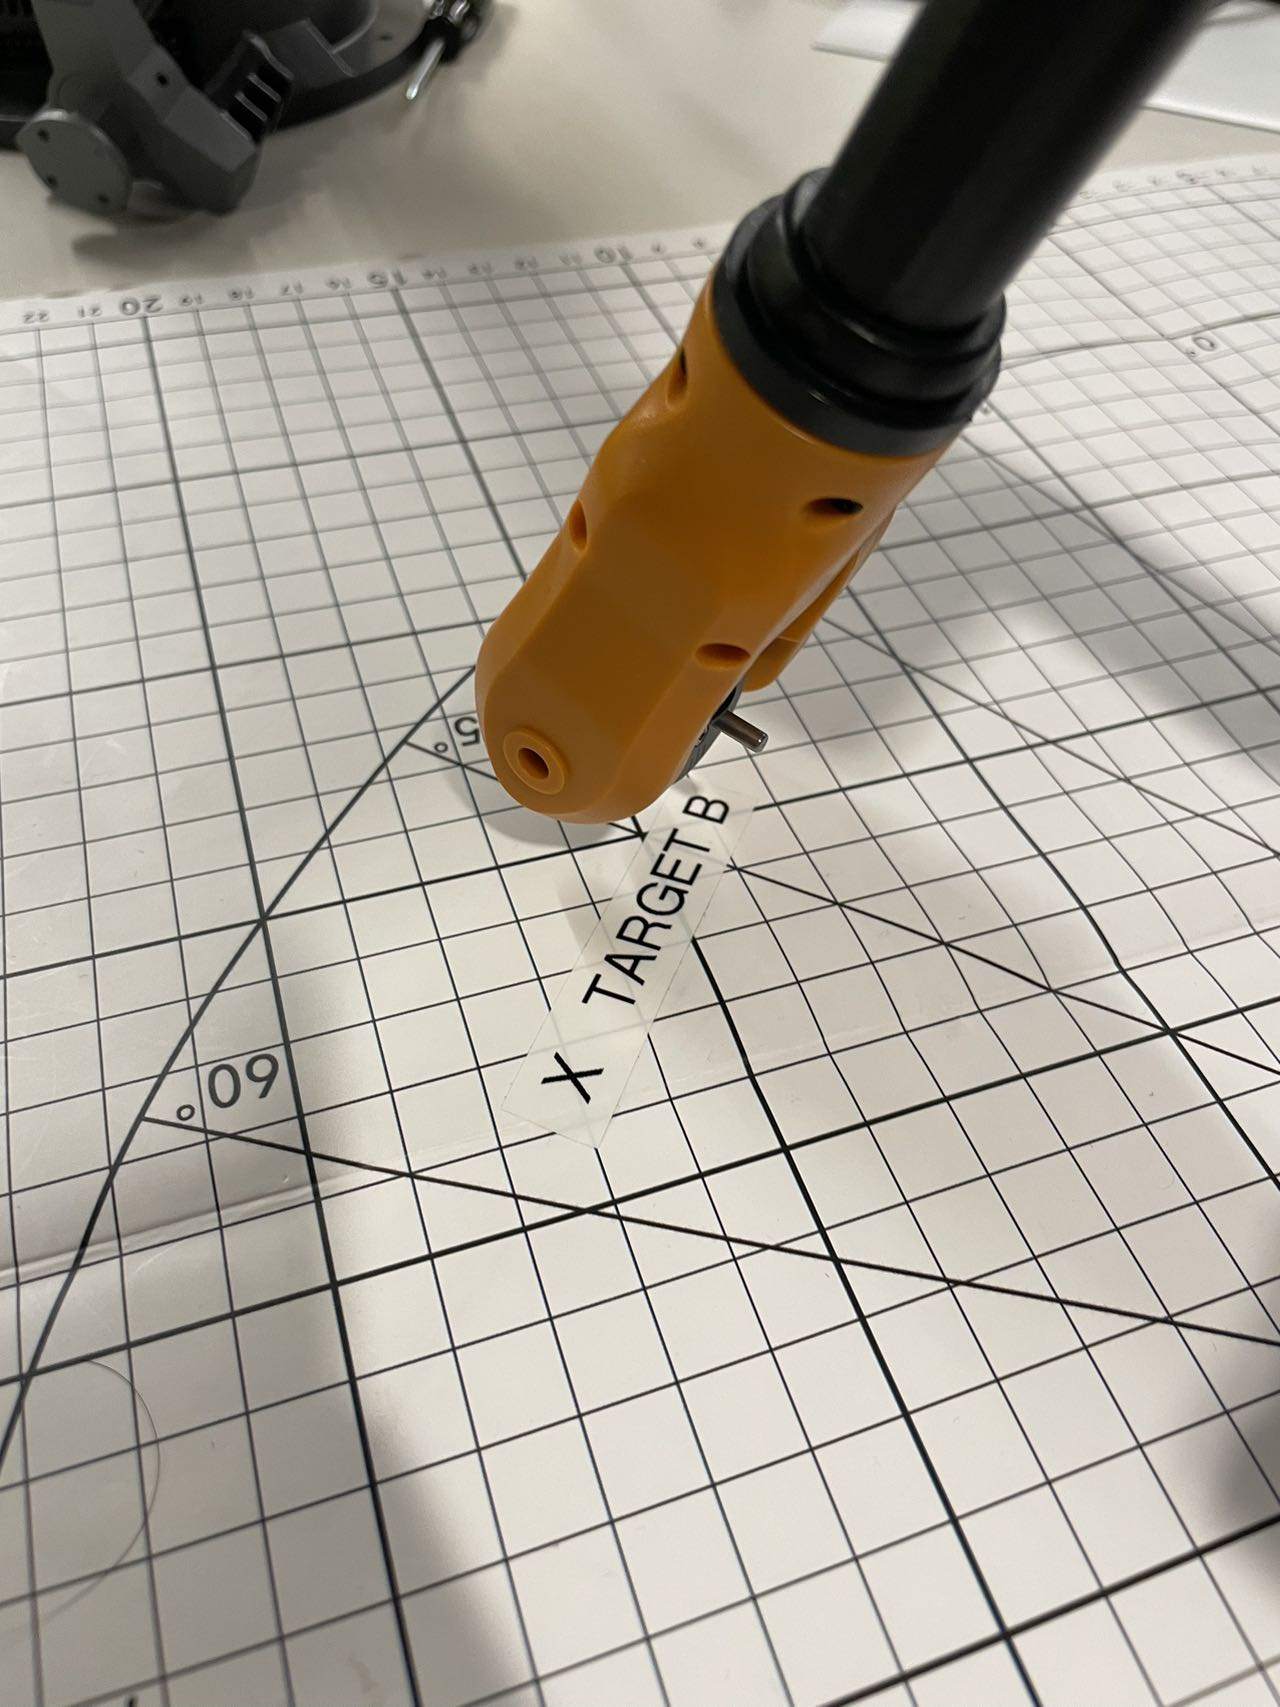
\includegraphics[height=2.5in]{image/4c_b.jpg}
\end{center}

\newpage
\paragraph{Additional Space.}
Please do not exceed this page for this question.
%%%%%% YOU ANSWER ENDS HERE
